\section{Design Patterns}
\subsection{Model View ViewModel (MVVM) Pattern}
\begin{figure}[H]
	\centering
	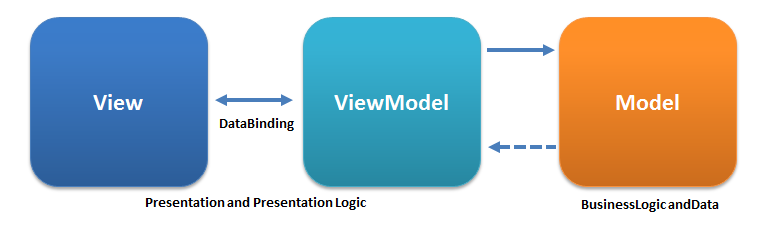
\includegraphics[scale=0.6]{Figures/WebImages/MVVMPattern}\\
	\caption{The MVVM Pattern - http://en.wikipedia.org/wiki/Model\_View\_ViewModel}
	\label{fig:MVVMPattern}
\end{figure}
The \texttt{DriveIT Windows Client} uses the "Model View ViewModel" architectural pattern which tries to ensure a clear separation between the model and the view. 
\subsection{Observer Pattern}

\subsection{Adapter Pattern}
The \texttt{DriveIT Windows Client} uses the \emph{Model View ViewModel} architectural pattern which tries to ensure a clear separation between the model and the view. The pattern derives from both the \emph{Model View Controller} pattern and the \emph{Presentation Model} design pattern and therefore has some of the same attributes. By using the MVVM pattern we created a more testable and easier expandable application. Furthermore we used \emph{Microsoft Blend}'s \emph{Behavior Actions} to encapsulate calls and commands from the View such that View elements would not get send to the ViewModel. These actions are implemented to ensure low coupling.\\

The adapter patterns allows the coder to encapsulate an object its methods and properties. The \texttt{DriveIT Windows Client} uses the MVVM design pattern originated from Microsoft, and it requires every view to have a corresponding Viewmodel, and furthermore The \texttt{DriveIT Web API} uses Data Transfer Objects(DTO) to send and receive data. Since DTO's are only meant to transfer data, no functions should exist in the class, therefore all Single Entitiy ViewModels in the \texttt{DriveIT.WindowsClient.ViewModels} name-space functions as Adapters for their corresponding DTO. E.g The CarViewModel class is an adapter for the CarDto class.\\ 

This implementation provides the WindowsClient with an easy way to manipulate data, while still retaining the data-structure such that it can be Created, Read, Updated and Deleted over the \texttt{DriveIT Web API} without converting.
\subsection{Observer pattern}
An important part of the "Model View ViewModel" pattern is the data-binding which exists between the View and their ViewModel, in WPF this is done by having the viewmodels implement the interface \texttt{INotifyPropertyChanged} which will notify the view when the ViewModel has changed. By using this interface the ViewModel knows nothing of the view and cannot directly change its attributes.

\subsection{Façade Pattern}
The facade design pattern is used several times in the \texttt{DriveIT System}.
The \texttt{Persistent Storage} sub system uses a facade pattern do hide the internal sub systems that accomplish the functionality defined in the \texttt{IPersistentStorage} interface.

The \texttt{DriveITContext} defined in the sub system is used by an implementer, \texttt{EntityStorage}, on the interface, but is hidden for users of the interface. 

\begin{figure}[H]
	\centering
	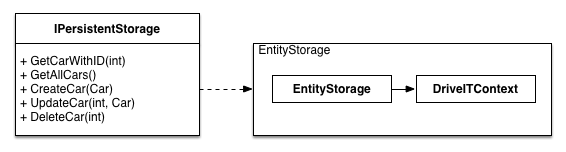
\includegraphics[scale=0.6]{Figures/FacadePatternPersistentStorage}\\
	% place the figure in the Figures folder (located with the main file)
	% you need to fix the scale a few times to get it right, but latex does not compress so one can always zoom in to see details.
	\caption{The Facade Pattern of IPersistentStorage.}
	\label{fig:The Facade Pattern of IPersistentStorage.}
	% label it something meanfull
\end{figure}
